\subsection{Builder Marketplace}
The Builder Marketplace is a next-generation ecosystem designed to streamline cross-chain communication for decentralized applications (dApps) by leveraging a network of modular solvers. These solvers integrate existing blockchain protocols across multiple chains, ensuring seamless interoperability and enhanced functionality for dApps. Our approach is unique in that we aggregate existing protocols from all blockchain networks and create modular representations of each dApp within our architecture. These dApp modules encapsulate all relevant information about a given application, enabling official teams to access, manage, and update their modules through a dedicated dashboard, similar to how APIs are managed and deployed on platforms like Postman today.

\begin{figure}[h]
    \centering
    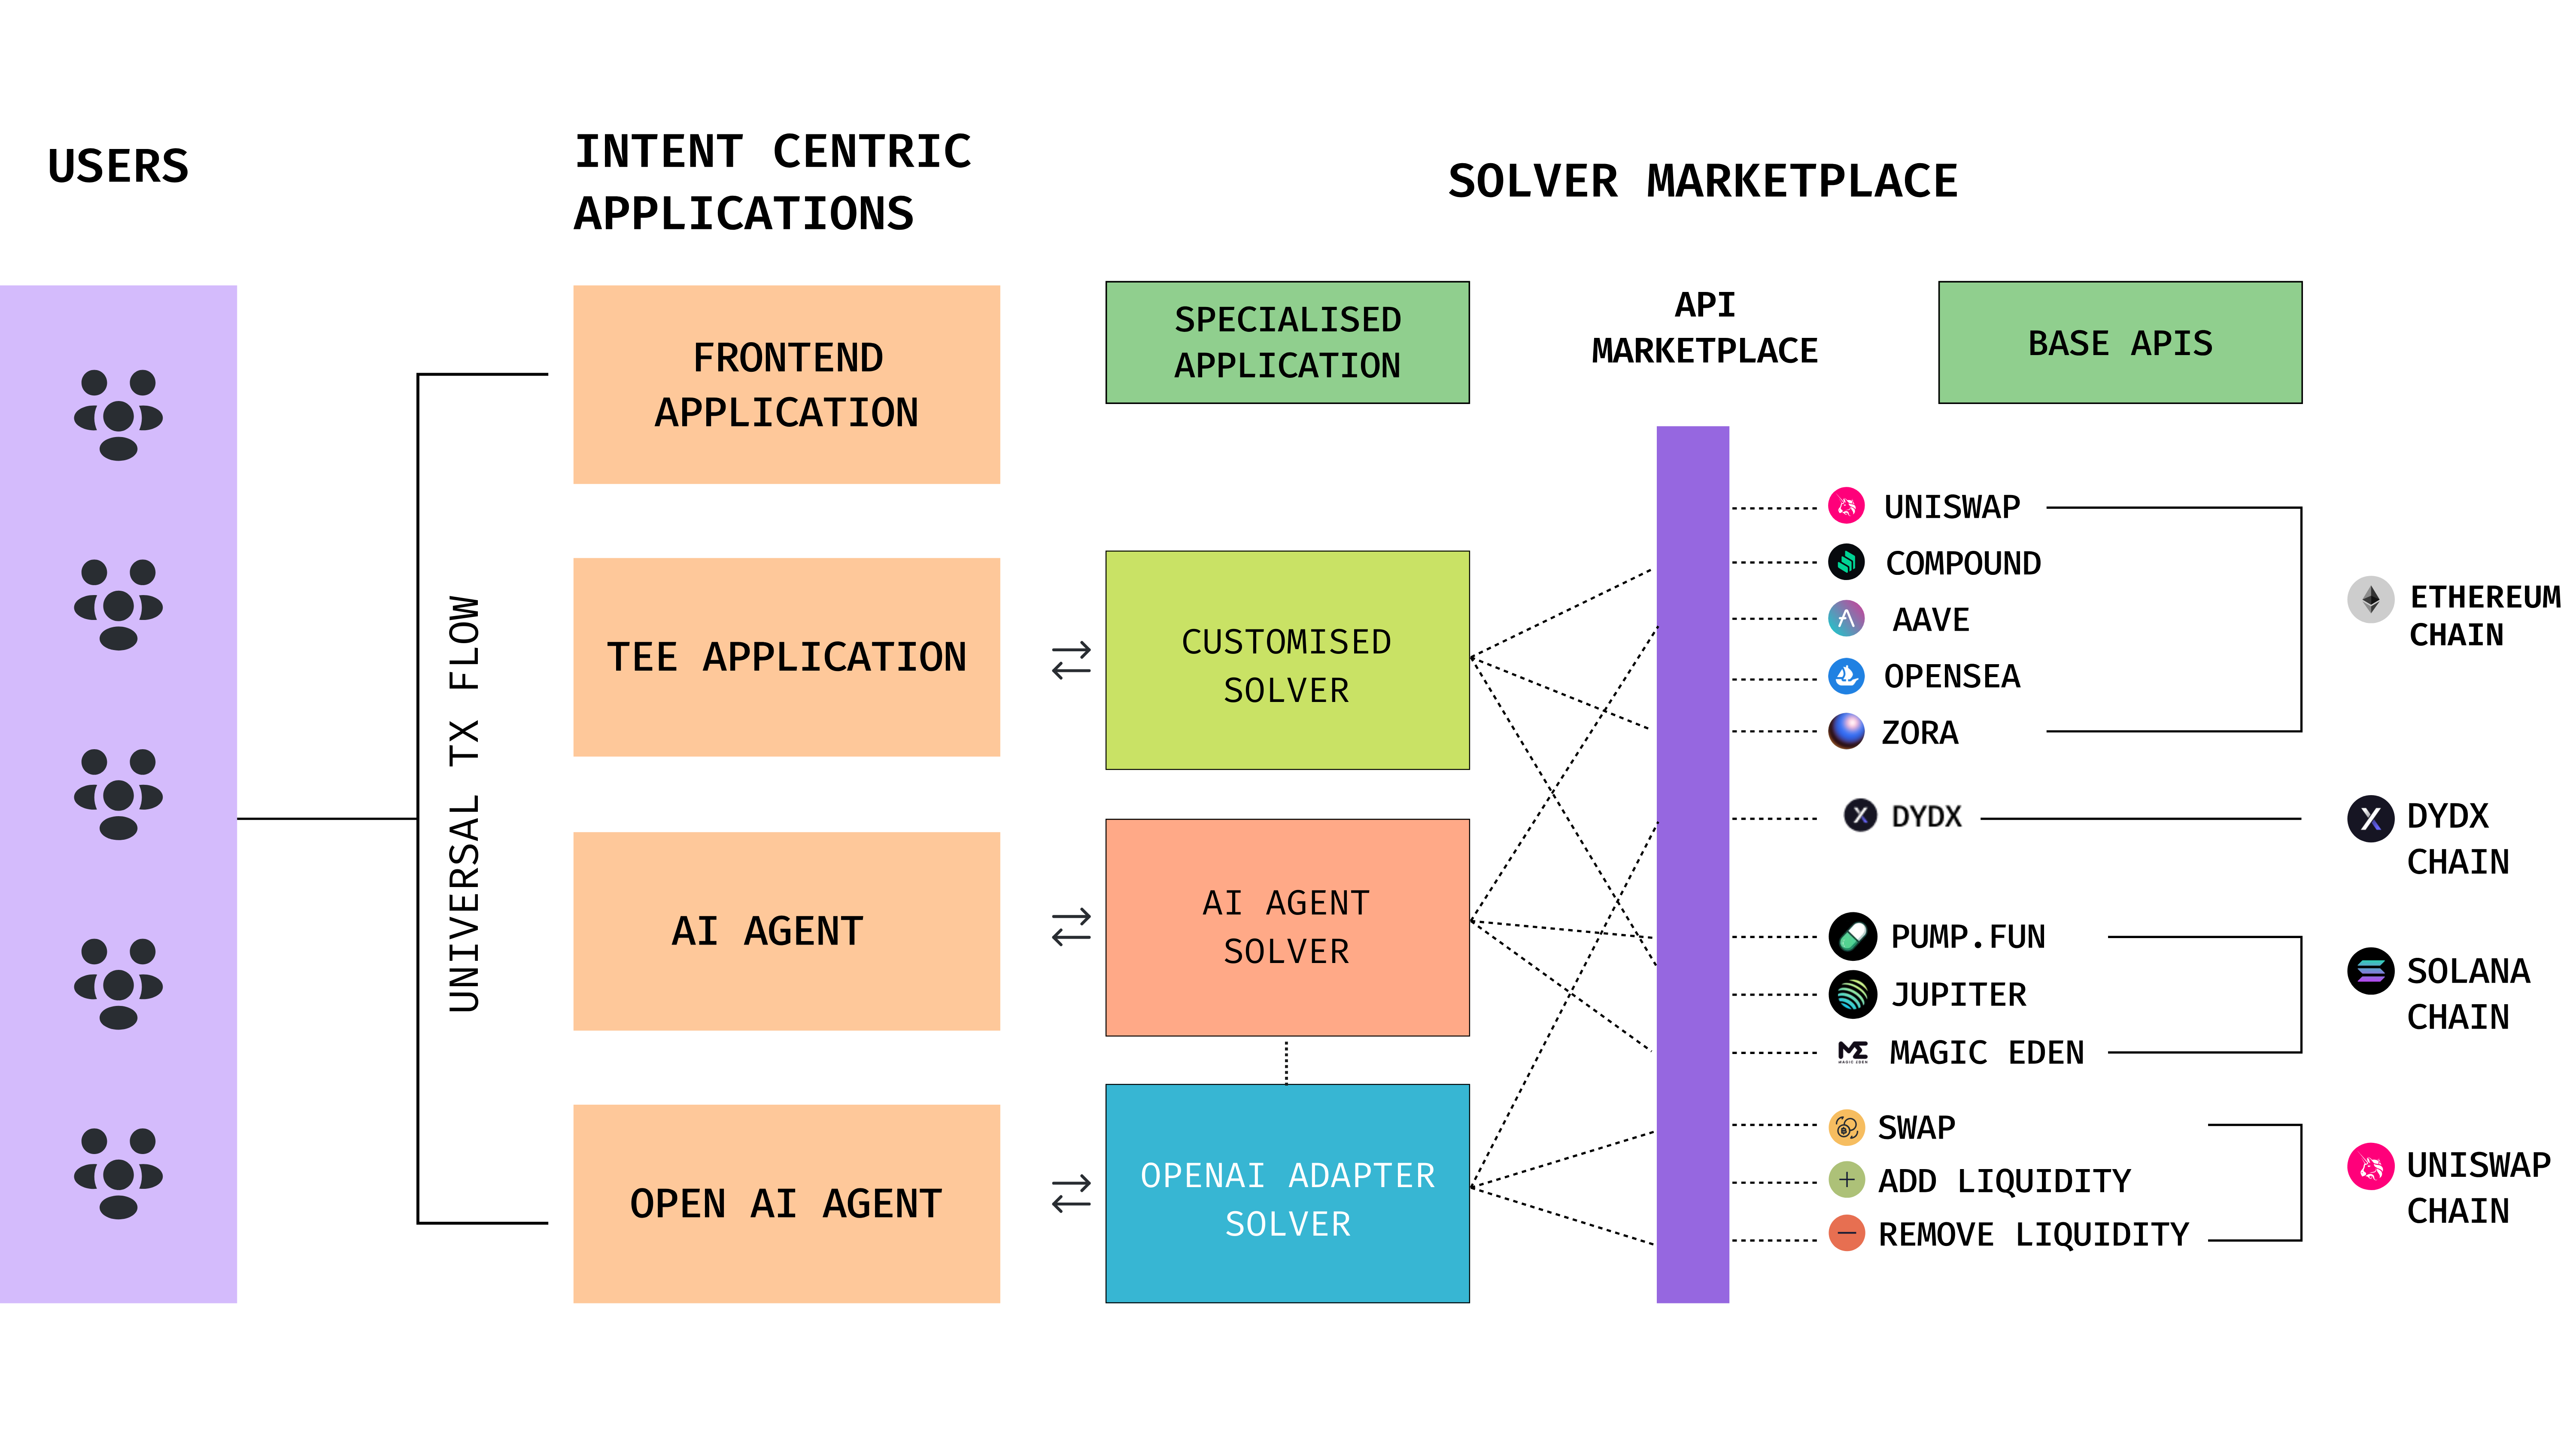
\includegraphics[width=0.9\linewidth]{figure/builder.png}
    \caption{Builder Marketplace Overview}
    \label{fig:builder}
\end{figure}

Beyond these dApp modules, developers can build customized solvers by merging functionalities from multiple modules. This allows for flexible and composable solutions, ensuring seamless cross-communication between solvers while optimizing execution paths. The Builder Marketplace supports universal transaction flows, catering to intent-centric applications, AI agents, and direct API calls from frontend applications. In addition, these specialized and base solvers feature dedicated interfaces, which can be used by intent-centric protocols and AI agents, further enhancing the interoperability, efficiency, and scalability of decentralized applications. By providing a structured yet adaptable framework, the Builder Marketplace serves as a powerful foundation for the next wave of blockchain-powered innovations.

By focusing on solver-driven execution, cross-chain interoperability, and a modular architecture, the Builder Marketplace empowers developers to create highly efficient and scalable solutions for decentralized applications. This ecosystem bridges the gap between disparate blockchain networks, offering a unified platform for seamless transaction execution and inter-chain communication.



\subsubsection{Intent Standardization}

To enable seamless cross-chain intent execution beyond Ethereum, ERC-7683 (Ethereum Cross-Chain Intent Standard) must be extended to support multiple Layer 1 (L1) chains. This requires a standardization layer that translates diverse intent formats from various chains into a unified standard intent format. The standard intent is then processed by a solver network, where each solver operates as an omni rollup and executes transactions across multiple L1s through chain-specific adapters.
\begin{figure}[h]
    \centering
    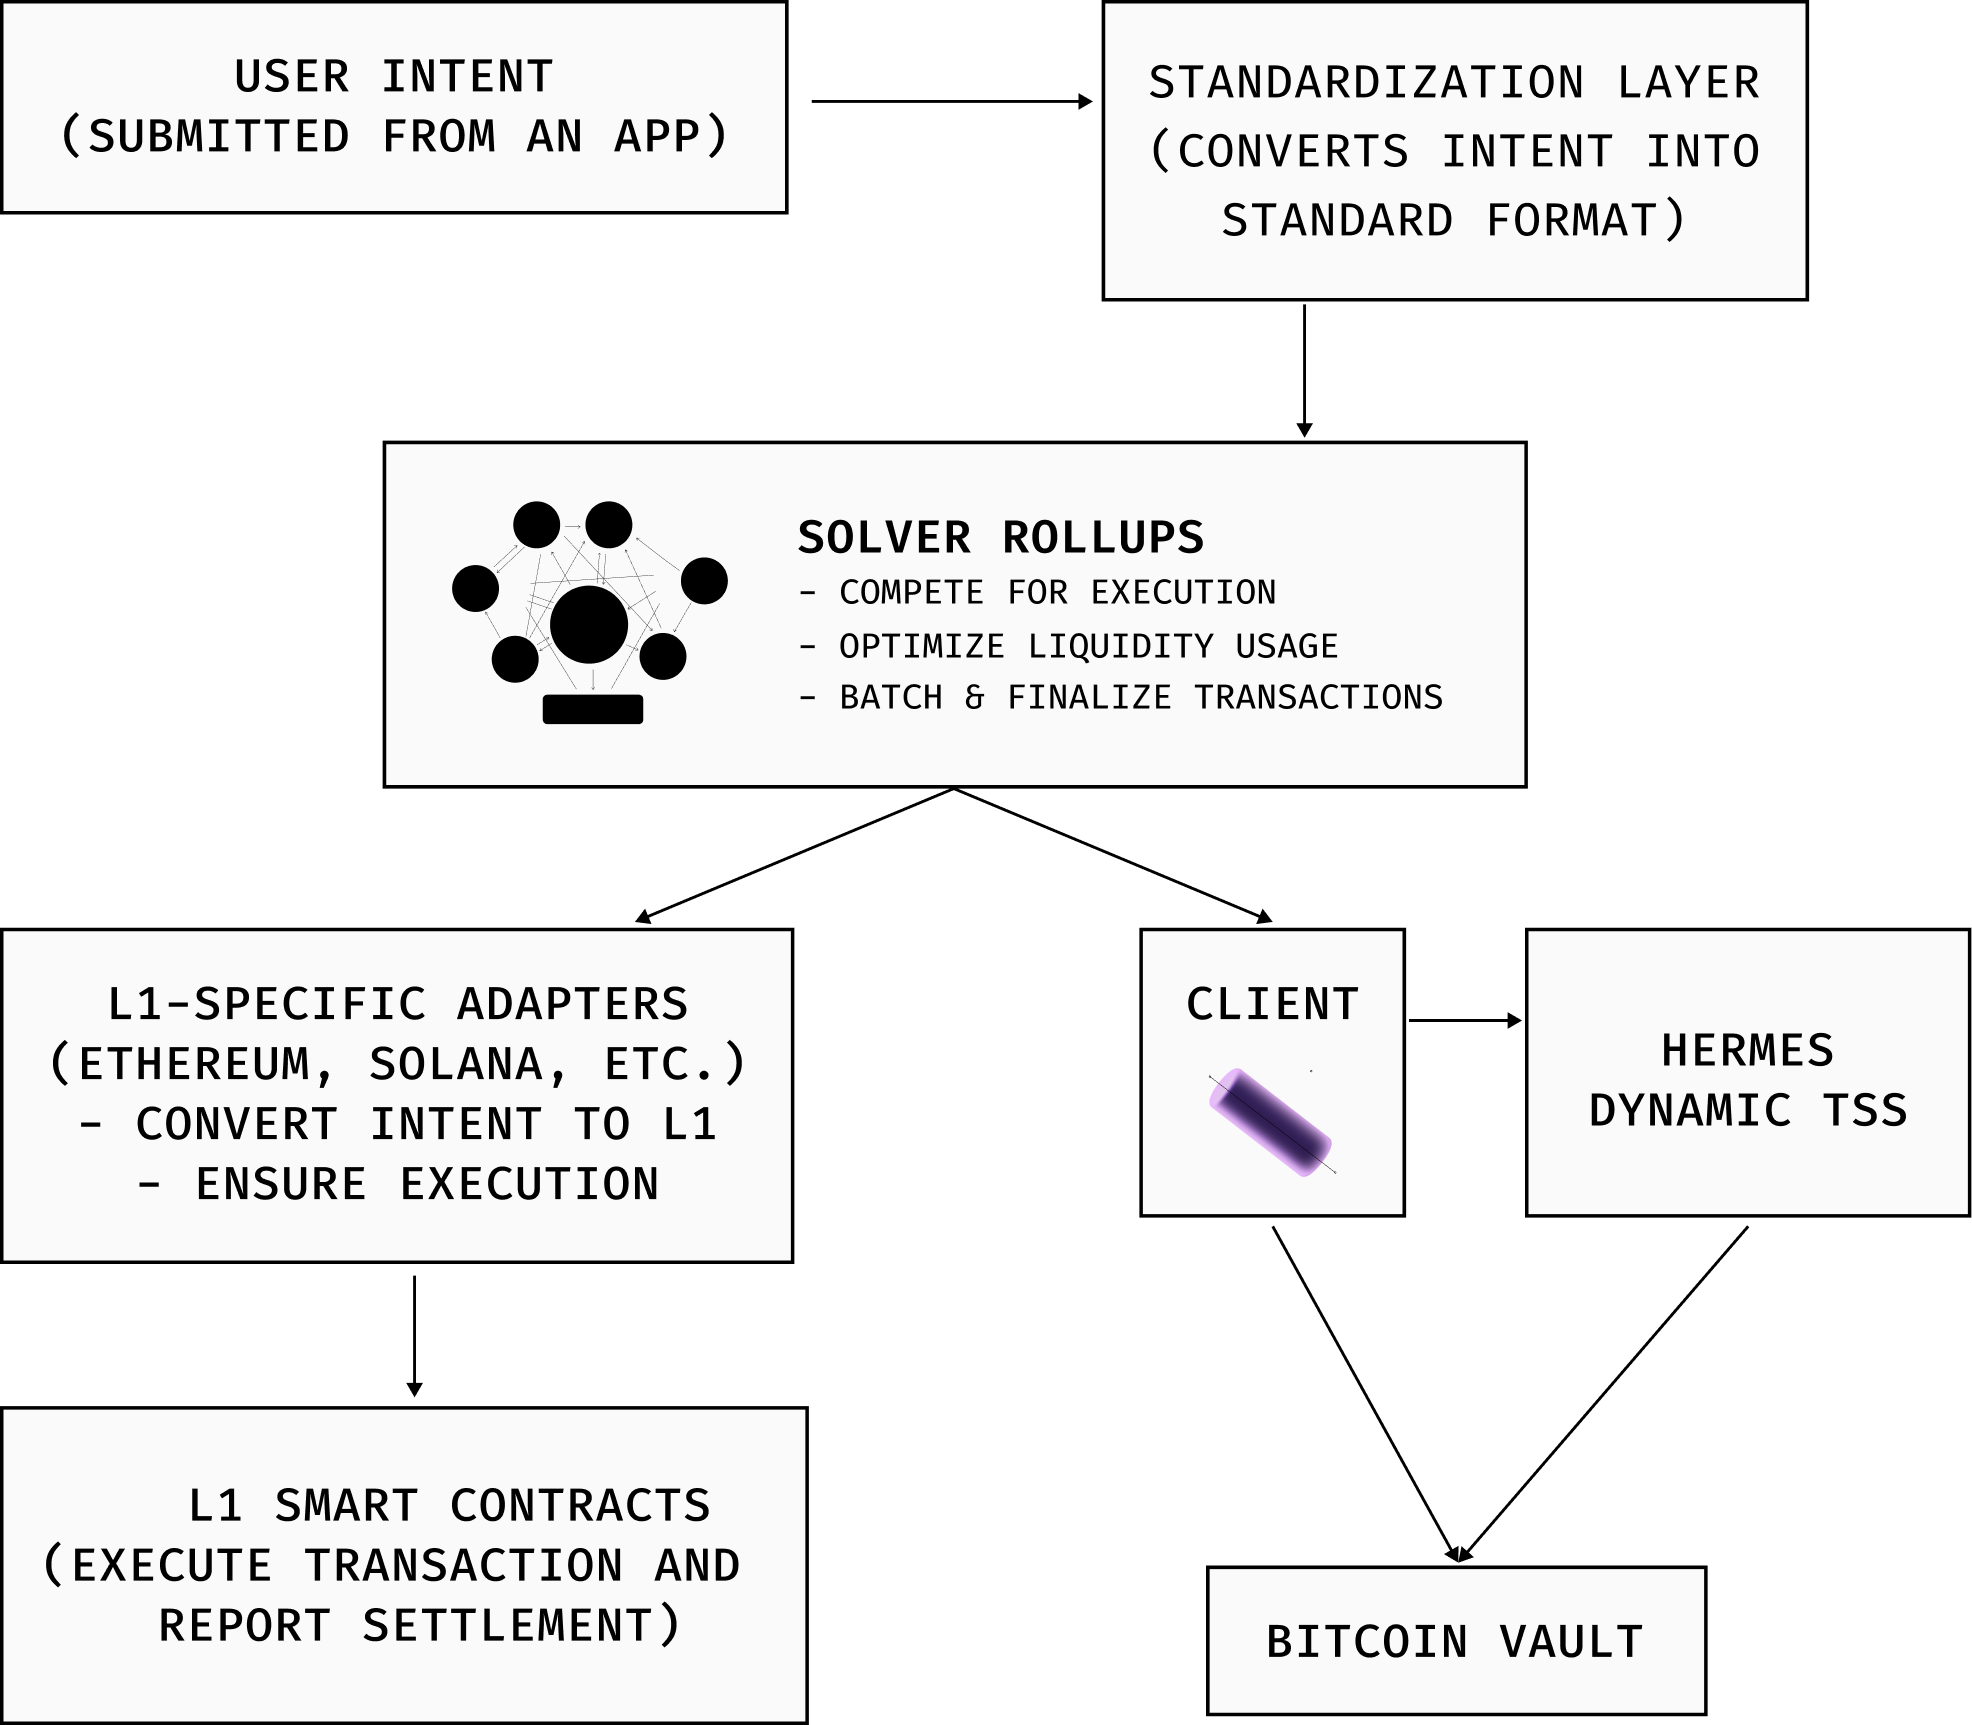
\includegraphics[width=0.9\linewidth]{figure/Intent.png}
    \caption{Intent Standardization Illustration}
    \label{fig:intent}
\end{figure}

\noindent
\textbf{Standardization Layer for Cross-Chain Intents}

The Standardization Layer acts as the universal interpreter for intents, ensuring that any user-submitted intent—whether from Ethereum, Solana, Avalanche, Cosmos, or other L1s—is converted into a common format. This allows solvers to process and optimize execution without being constrained by chain-specific differences.

The unified intent format will include:

-   Intent Type: Swap, bridge, stake, borrow, lend, liquidate, etc.

-   Source and Destination Chains
    
-   Assets and Amounts
    
-   Execution Preferences: Slippage tolerance, gas fee preferences, execution deadline
    
-   Security Conditions: Required confirmations, fraud-proof verification, authentication

The conversion process is handled through intelligent parsers that extract intent data from L1-native formats (such as Ethereum calldata, Solana transaction instructions, or Cosmos IBC packets) and translate it into the standardized format.

\noindent
\textbf{Chain-Specific Adapters for Execution on L1s}

Once the intent is standardized, it needs to be executed according to the transaction rules of the target L1. This is where L1-specific adapters come into play. These adapters translate the standardized intent into an L1-compatible transaction, ensuring compliance with that blockchain's smart contract execution model, fee structure, and consensus rules.

For example:

    On Ethereum, the adapter converts the standardized intent into an ERC-7683-compatible calldata format to be executed via smart contract calls.
    On Solana, the adapter translates it into Solana Program Instructions (SPI), ensuring compatibility with Solana’s account-based execution.
    On Cosmos, the adapter formats it into IBC messages, enabling cross-zone transactions.
    On Avalanche, it transforms the intent into Subnets-compatible transactions.

Each L1 maintains a solver contract that listens for execution instructions from the solver rollup. The solver contract executes the translated intent and reports the transaction status back to the solver network, which finalizes the process.

Since each solver operates as an omni rollup, it serves as both an executor and liquidity provider. These solvers: Process standardized intents and optimize execution routes. Communicate with L1 adapters to ensure successful execution. Manage liquidity pools on L1s via smart contracts. Aggregate and batch transactions before settlement, reducing on-chain congestion.
This ensures efficient execution of the intent across the chain, while also reducing gas costs by using Omnichain Web’s roll-up infrastructure.
\begin{figure}[h]
    \centering
    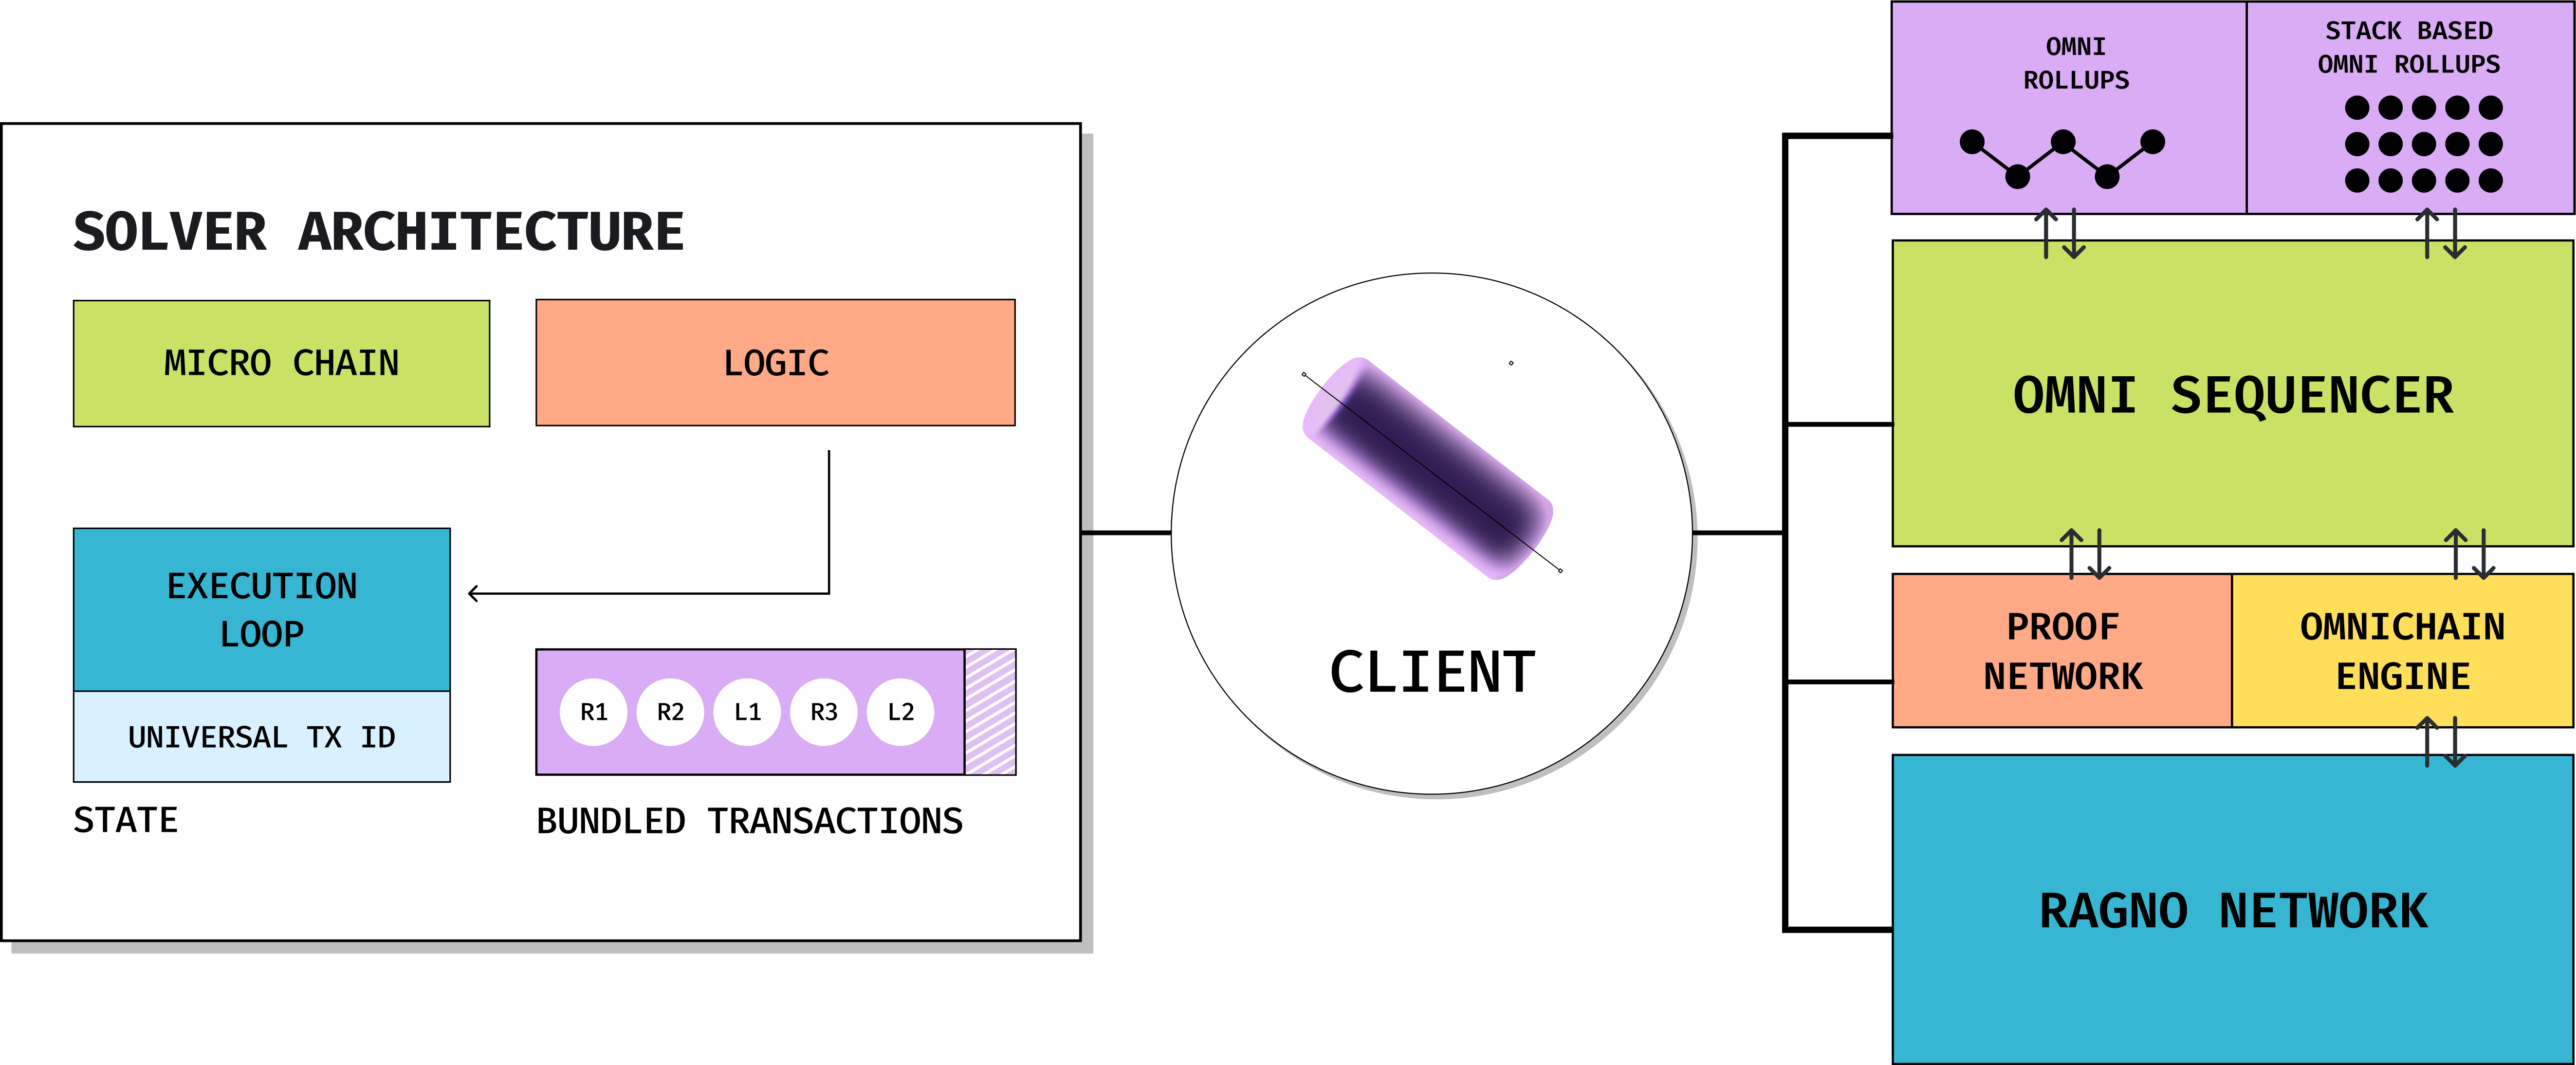
\includegraphics[width=0.9\linewidth]{figure/solver.png}
    \caption{Solver Illlustration}
    \label{fig:solver}
\end{figure}

\subsubsection{Solver Network}
The Solver Network is a peer-to-peer collaborative network of omni-rollup solvers, each operating independently while cooperating dynamically to optimize intent execution. Each solver is deployed as an omnirollup, ensuring scalability, decentralization, and security. The network supports both simple and complex intents, leveraging netting mechanisms and liquidity rebalancing to enhance execution efficiency while minimizing capital lockup.

Each solver runs its own Linera microchain~\cite{linera} based omni rollup, enabling independent processing of intents while maintaining full interoperability across the Solver Network. Each microchain consists of: Rust-based execution logic for handling transactions. Cross-chain address management to interact with various blockchains. Base API services for mempool scanning, netting, and solver coordination.

\begin{figure}[h]
    \centering
    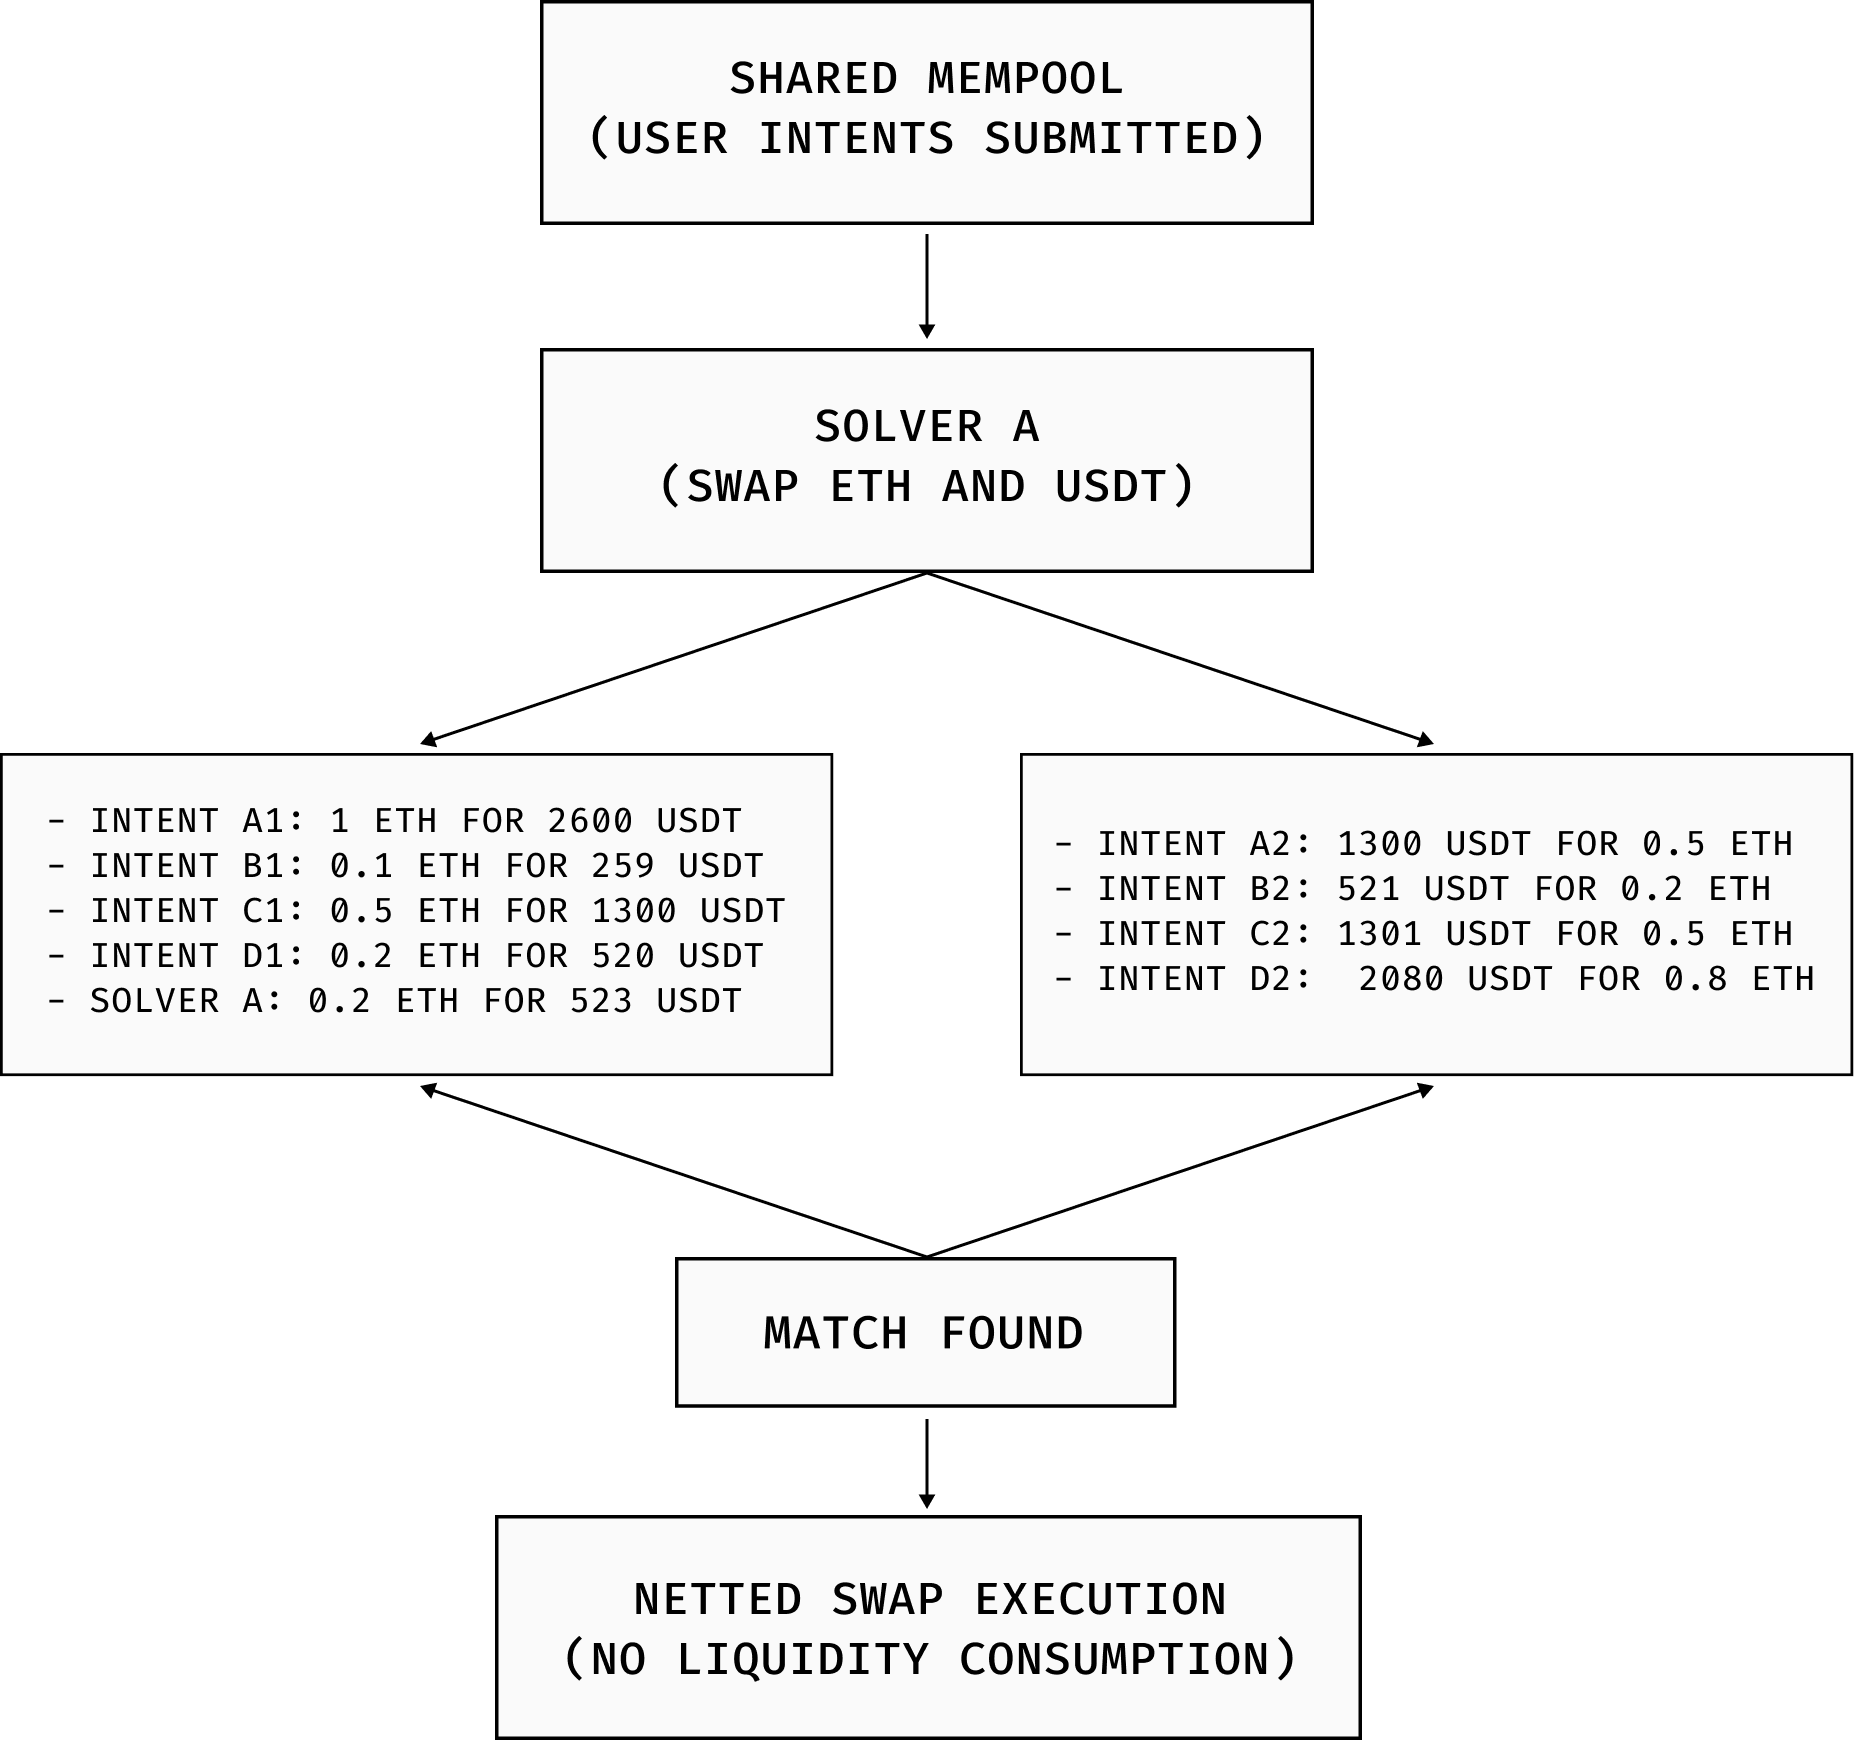
\includegraphics[width=0.9\linewidth]{figure/Netting.png}
    \caption{Netting Process}
    \label{fig:netting}
\end{figure}

\textbf{Peer-to-Peer Solver Collaboration and Netting System}

Unlike traditional execution models that rely on direct liquidity consumption, the Solver Network first attempts to net out user intents before executing them on-chain. This is achieved by matching complementary intents in a shared mempool, reducing the reliance on external liquidity. For example: If User A submits an intent to swap ETH → USDC, and User B submits an intent to swap USDC → ETH, solvers can net these transactions out internally, allowing A and B to swap without affecting liquidity reserves. More complex intents—such as multi-hop swaps, cross-chain arbitrage, and lending liquidations—can be batched into netted sets where one set of transactions offsets the other. Each netted batch is designed to minimize slippage, reduce gas fees, and optimize execution.

Solvers continuously scan the mempool to find optimal netting opportunities, ensuring that user intents are fulfilled with minimal external liquidity impact. If netting is not possible, solvers proceed with direct execution using their available liquidity or by coordinating with other solvers.

\begin{figure}[h]
    \centering
    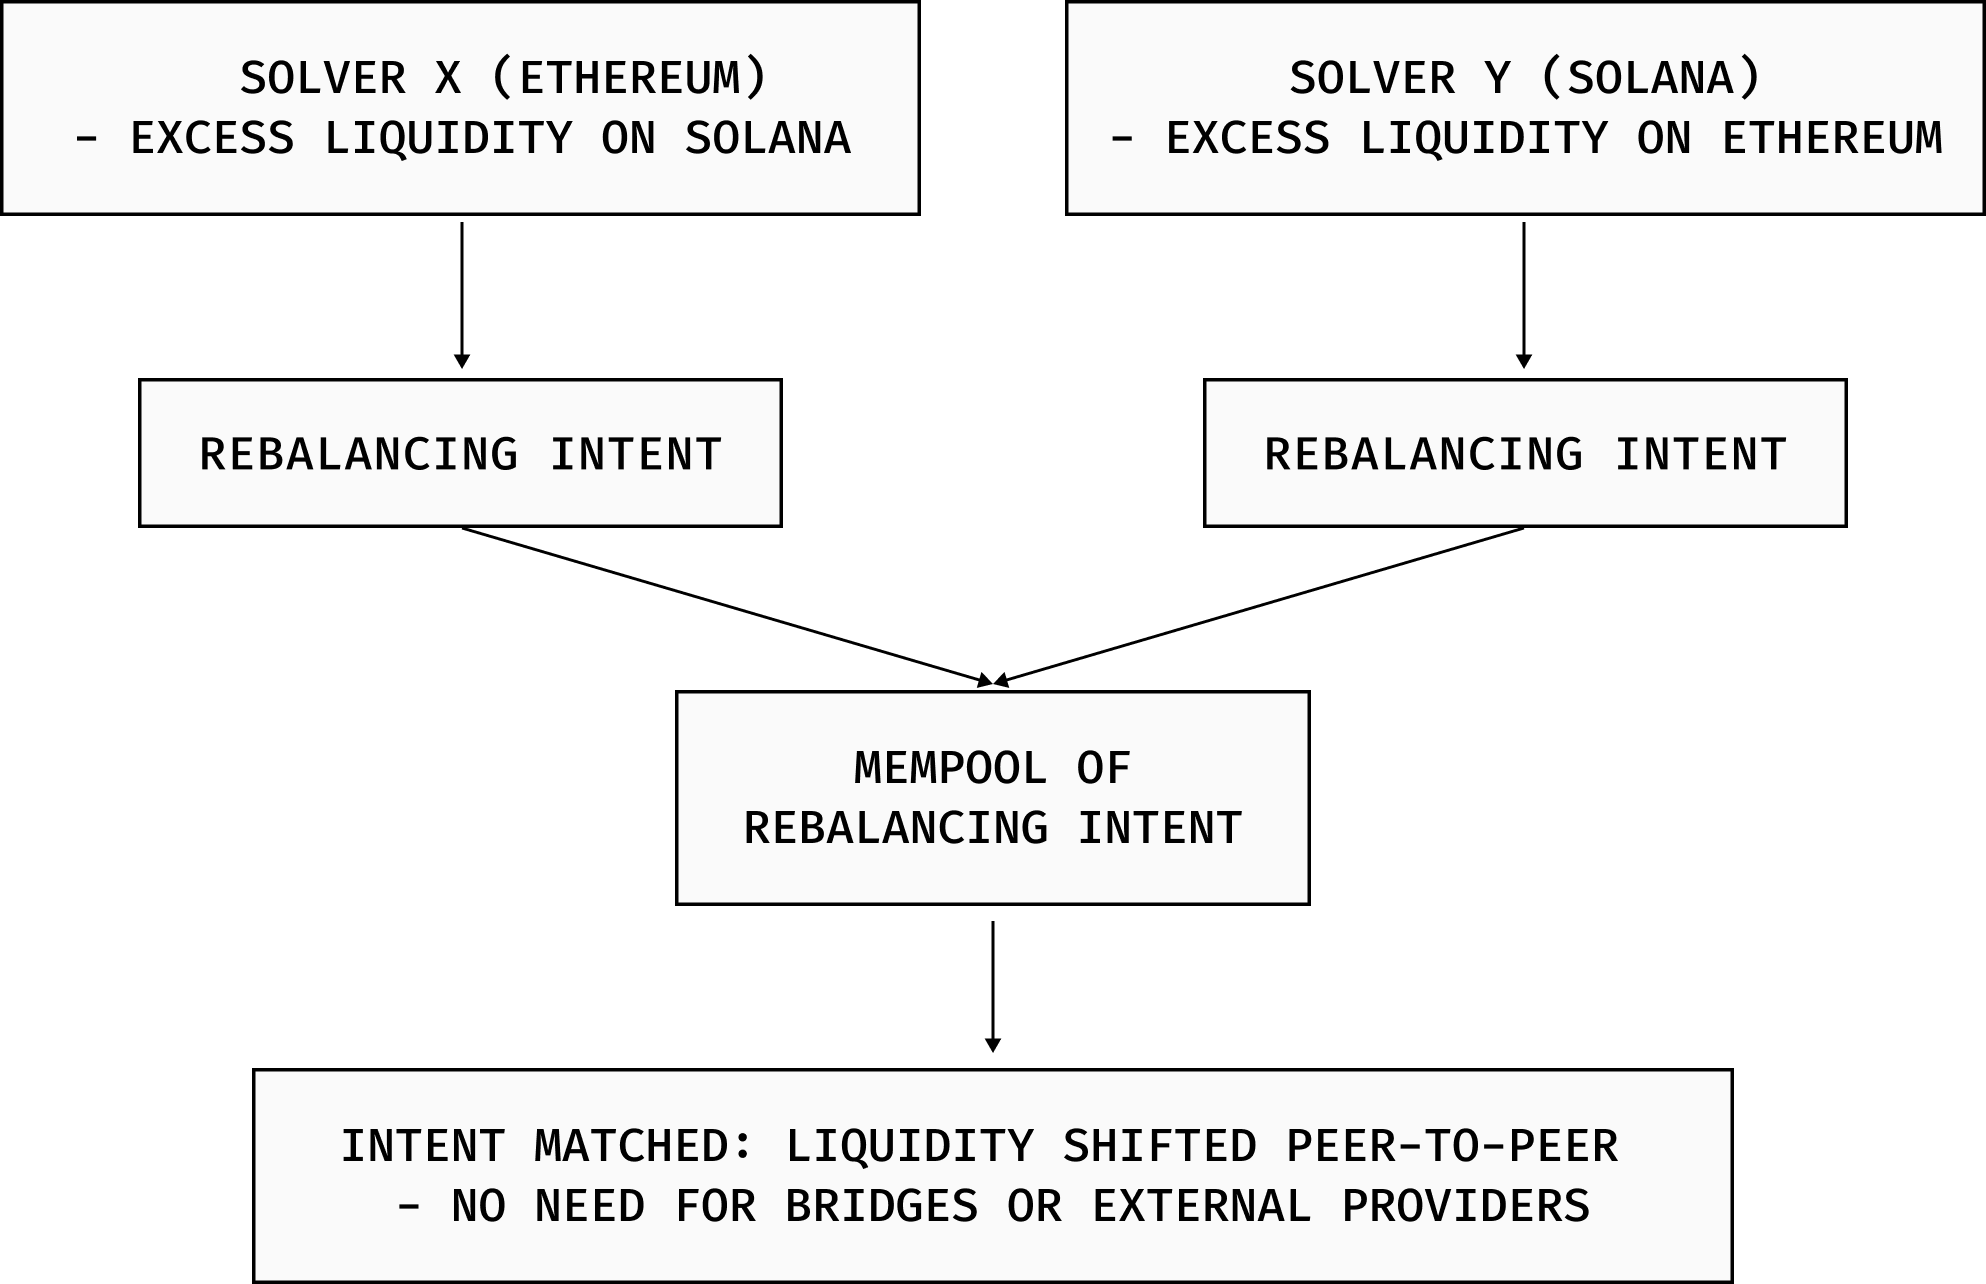
\includegraphics[width=0.9\linewidth]{figure/Rebalancing.png}
    \caption{Rebalancing Illustration}
    \label{fig:rebalancing}
\end{figure}

\textbf{Liquidity Rebalancing Through Intent Generation}

Solvers manage their own liquidity across multiple chains, but maintaining balance across different ecosystems is challenging. To prevent inactive liquidity buildup, solvers proactively generate rebalancing intents, which are fulfilled by other solvers that need opposite liquidity shifts.

Example scenario: Solver X (Ethereum) has excess liquidity on Solana but wants to move it back to Ethereum. Solver Y (Solana) has excess liquidity in Ethereum and wants to move it to Solana.
Instead of using bridges or external liquidity providers, Solver X and Solver Y fulfill each other's rebalancing intents, ensuring that both solvers retain liquidity within their own systems. This decentralized liquidity rebalancing mechanism improves capital efficiency, prevents unnecessary fragmentation, and reduces reliance on traditional liquidity bridges, which are prone to delays and security risks.



\subsubsection{Transaction Flow}
The transaction flow in the Builder Marketplace is designed to accommodate multiple types of transactions, ensuring seamless execution from the initiation to the final settlement. The different types of transaction include intent-centric transactions, AI-driven transactions, and direct API call transactions. Below is a breakdown of the transaction flow:
\begin{itemize}
    \item \textbf{Transaction Initiation}:

    Transactions can be initiated through intent-centric applications, AI agents, or direct API calls from front-end applications. Once a transaction request is submitted, the solver network analyzes it and determines the most efficient execution route.

    \item \textbf{Solver Selection and Processing}:

    The appropriate solver or group of solvers is chosen based on the characteristics of the transaction. They validate the transaction by verifying the input dependencies and feasibility. Cryptographic signatures are used to ensure authenticity. Solvers analyze pending intents and attempt netting optimizations. If netting is insufficient, solvers coordinate execution using peer-to-peer liquidity sharing.
    Solvers bundle transactions and send them to the Omni Sequencer for ordering.

    \item \textbf{Cross-Chain Communication and Execution}:

    For cross-chain transactions, the solvers communicate through the microchain structure, utilizing integrated blockchain protocols for efficient execution. When omni-rollup handling is required, solvers bundle the transaction and forward it to the Omni Sequencer, which organizes and submits it to the appropriate rollup for execution.

    \item \textbf{Finalization and Settlement}:

    For omni-rollup transactions, the solver network monitors transaction progress, providing pre-confirmation and final confirmation updates. In the case of direct Layer 1 (L1) settlements, the solver collaborates with Hermes validators to execute the transaction. The final transaction state is then recorded on the relevant blockchain, ensuring both transparency and immutability.
    
    \item \textbf{Confirmation and Feedback}:
    
    Users receive updates on transaction status in real time through the interface of the solver network. The system is designed to ensure efficient and secure transaction completion, optimizing minimal latency while maintaining maximum security.
\end{itemize}

    
This structured transaction flow ensures that the Builder Marketplace efficiently handles a diverse range of transactions while maintaining high performance, security, and scalability.